\documentclass{ximera}

\title{Graphing Activity Solutions Guide}
\author{MATH 425: Calculus I}

\begin{document}
\begin{abstract}
    Working with the peers in your group, solve the following problems. Make sure to show and justify all your work. Make sure everyone in the group understands the solution and participates. Be prepared to report your answers to the whole class. 
\end{abstract}
\maketitle


\begin{exercise}
    Determine if any of the following statements are true or false.  Explain your reasoning. (If your answer is false, an example may be enough explanation.  If your answer is true, an example is not enough.)
    \begin{enumerate}
        \item Every relative maximum and minimum of a function $h$ occurs at a point $c$ where $h'(c)$ is either zero or does not exist.\\
        This statement is \textcolor{blue}{TRUE}  because \dots\\
        \textcolor{blue}{This is the definition of a critical points.  We know that any relative minimum or maximum must occur at a critical point of the function. }
        \item At every point $c$ where $h'(c)$ is zero or does not exist, the function $h$ has a relative maximum or minimum.\\
        This statement is \textcolor{blue}{FALSE} because \dots\\
        \textcolor{blue}{Counterexample: $f(x)=x^{\frac{1}{3}}$ has no relative minimum or maximum values.\\
        $f'(x)=\frac{1}{3}x^{-\frac23}$, and $f'(0)$ does not exist.  However, this is not a relative maximum or minimum of the function.}
    \end{enumerate}
\end{exercise}

\begin{exercise}
    Suppose that $g(x)$ is a function that is continuous for every value of $x\neq 2$ whose first derivative is 
    $$g'(x)=\frac{(x+4)(x-1)(2x-2)}{x-2}.$$
    Further, note that $g$ has a vertical asymptote at $x=2$. 
    \begin{enumerate}
        \item Determine all critical numbers of $g(x)$.\\
        \textcolor{blue}{We need to set $g'(x)=0$ and find any values where $g'$ does not exist. \\
        $x=2$ causes division by zero (found by setting $x-2=0$), so $g'$ does not exist.\\
        $g'(x)=0$ when the numerator is zero: 
        \[(x+4)(x-1)(2x-2)=0\]
        $x=-4, 1$ are where $g'(x)=0$.\\
        Critical numbers: $x=-4,1,2$}
        \item By developing a carefully labeled first derivative sign chart, decide whether $g(x)$ has a local maximum, local minimum, or neither at each critical number.\\
        \textcolor{blue}{
          \begin{tabular}{c|c|c|c}
            $(-\infty,-4)$ & $(-4,1)$ & $(1,2)$ & $(2,\infty)$\\
            $+$ & $-$ & $-$ & $+$
          \end{tabular}
          Choose a test point in each interval to determine these signs, for example:\\
          $g'(-5)=\frac{(-5+4)(-5-1)(2(-5)-2)}{-5-2}=\frac{72}{7}$\\
          $g'(0)=\frac{(0+4)(0-1)(2(0)-2)}{0-2}=-4$\\
          $g'(0.5)=\frac{(0.5+4)(0.5-1)(2(0.5)-2)}{0.5-2}=-\frac32$\\
          $g'(3)=\frac{(3+4)(3-1)(2(3)-2)}{3-2}=56$\\
          $x=-4$ is a local maximum.  No local minimum, since $x=2$ is an asymptote.
        }
        \item Does $g$ have a global maximum?  Global minimum?  Justify your claims.\\
        \textcolor{blue}{Having an asymptote means that on at least one side of the asymptote the function is approaching infinity.  Based on the sign diagram, the function is increasing as it approaches 2 from the left (namely, going to $-\infty$). Therefore, it cannot have a global min.  The function is also increasing to $\infty$ as x gets larger after $x=2$, so there is no global max. }
        \item Sketch a possible graph of $y=g(x)$. (Focus on shape rather than exact points included on the graph.)
        \begin{image}
          \includegraphics{graphing1A.png}
          %\xmalt{A sketch of a graph that is increasing and concave down until $x=-4$, decreasing and concave down until $x=1$ and again until approaching $x=2$ (the graph goes flatish at $x=1$ to show the derivative is 0 at $x=1$).  At $x=2$ there is a dashed vertical line indicating the asymptote.  The graph then increases from after $x=2$ onwards. }

            %\begin{tikzpicture}
  %\begin{axis}[
    %axis lines=middle,
    %xlabel={$x$},
    %ylabel={$y$},
    %xmin=-5, xmax=5,
    %ymin=-5, ymax=5,
    %grid=both,
    %minor tick num=1,
    %axis equal image,
    %view={0}{90},
  %]

  %\end{axis}
%\end{tikzpicture}
        \end{image}
    \end{enumerate}
\end{exercise}

\begin{exercise}
    Suppose that $g$ is a function whose second derivative $g''$ is given by the graph below. 
    \begin{image}
        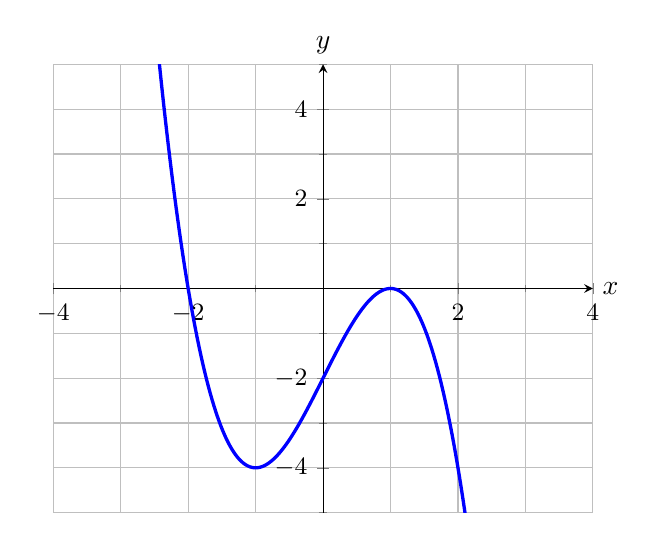
\begin{tikzpicture}
  \begin{axis}[
    axis lines = middle,
    xlabel = {$x$},
    ylabel = {$y$},
    xmin = -4, xmax = 4,
    ymin = -5, ymax = 5,
    grid = both,
    minor tick num = 1,
    ticklabel style={font=\small},
    every axis x label/.style={at={(current axis.right of origin)}, anchor=west},
    every axis y label/.style={at={(current axis.above origin)}, anchor=south},
  ]

    % Graph of y = -(x-1)^2(x+2)
    \addplot[
      domain=-4:4,
      samples=300,
      very thick,
      blue,
    ]
    { -((x - 1)^2) * (x + 2) };

  \end{axis}
\end{tikzpicture}
    \end{image}
       %\xmalt{A graph of what looks like a cubic polynomial with negative leading coefficient. Direction changes at the points $(-1,-4)$ and $(1,0)$.  Zeros of the graph are at $(-2,0)$ and $(1,0)$.  The $y$-intercept is at $(0,-2)$. }
    \begin{enumerate}
         \item Find the $x$-coordinates of all points of inflection for $g$.\\
         \textcolor{blue}{$x=-2$ is the only point of inflection.  $g''(x)=0$ when $x=0$ as well, but the sign does not change.} 
    \item Fully describe the concavity of $g$ by making an appropriate sign chart.\\
      \textcolor{blue}{\begin{tabular}{c|c|c}
        $(-\infty,-2)$ & $(-2,0)$ & $(0,\infty)$\\
        $+$ & $-$ & $-$
      \end{tabular}
      Concave up on $(-\infty,-2)$ and concave down on $(-2,0)$ and $(0,\infty)$.
      }
    \item Suppose you are given the information that $g'(-2)=0$.  Is there a local maximum, local minumum, or neither for the function $g$ at this critical number, or is it impossible to say?  why?\\
    \textcolor{blue}{The second derivative test is inconclusive here, as $g''(-2)=0$.  We cannot tell from this whether we have a max, min or neither.  However, we know that $g'(x)$ will have a local max at $x=-2$, as its derivative $g''$ changes sign at this point.  Therefore, $g'$ will not change signs at $x=-2$ and therefore cannot be a local max or min.}
    \item Assuming that $g''(x)$ is a polynomial (and that all important behavior of $g''$ is seen in the graph above). what degree polynomial do you think $g(x)$ is?  Why?\\
    \textcolor{blue}{It appears that $g''$ is a third degree (cubic) polynomial, so $g'$ would be 4th degree, and $g$ itself would be 5th degree.}
    \end{enumerate}
   
\end{exercise}





\end{document}